\documentclass[10pt]{beamer}

\usetheme[
%%% options passed to the outer theme
%    hidetitle,           % hide the (short) title in the sidebar
%    hideauthor,          % hide the (short) author in the sidebar
%    hideinstitute,       % hide the (short) institute in the bottom of the sidebar
%    shownavsym,          % show the navigation symbols
%    width=2cm,           % width of the sidebar (default is 2 cm)
%    hideothersubsections,% hide all subsections but the subsections in the current section
%    hideallsubsections,  % hide all subsections
    left               % right of left position of sidebar (default is right)
%%% options passed to the color theme
%    lightheaderbg,       % use a light header background
  ]{AAUsidebar}

% If you want to change the colors of the various elements in the theme, edit and uncomment the following lines
% Change the bar and sidebar colors:
%\setbeamercolor{AAUsidebar}{fg=red!20,bg=red}
%\setbeamercolor{sidebar}{bg=red!20}
% Change the color of the structural elements:
%\setbeamercolor{structure}{fg=red}
% Change the frame title text color:
%\setbeamercolor{frametitle}{fg=blue}
% Change the normal text color background:
%\setbeamercolor{normal text}{bg=gray!10}
% ... and you can of course change a lot more - see the beamer user manual.


\usepackage[utf8]{inputenc}
\usepackage[english]{babel}
\usepackage[T1]{fontenc}
% Or whatever. Note that the encoding and the font should match. If T1
% does not look nice, try deleting the line with the fontenc.
\usepackage{helvet}

\usepackage{subcaption}
\captionsetup{compatibility=false}

% colored hyperlinks
\newcommand{\chref}[2]{%
  \href{#1}{{\usebeamercolor[bg]{AAUsidebar}#2}}%
}


\date{\today}


	\title{sw608f14 - Piktotegner}
	\author{Daniel S. F, Lars A, Mathias W. P. \& Søren S. A.}
% - Give the names in the same order as they appear in the paper.
% - Use the \inst{?} command only if the authors have different
%   affiliation. See the beamer manual for an example

\institute[
%  {\includegraphics[scale=0.2]{aau_segl}}\\ %insert a company, department or university logo
  Dept.\ of Computer Science\\
  Aalborg University\\
  Denmark
] % optional - is placed in the bottom of the sidebar on every slide
{% is placed on the title page
  Department of Computer Science\\
  Aalborg University\\
  Denmark
  
  %there must be an empty line above this line - otherwise some unwanted space is added between the university and the country (I do not know why;( )
}


% specify a logo on the titlepage (you can specify additional logos an include them in 
% institute command below
\pgfdeclareimage[height=1.5cm]{titlepagelogo}{AAUgraphics/aau_logo_new} % placed on the title page
%\pgfdeclareimage[height=1.5cm]{titlepagelogo2}{graphics/aau_logo_new} % placed on the title page
\titlegraphic{% is placed on the bottom of the title page
  \pgfuseimage{titlepagelogo}
%  \hspace{1cm}\pgfuseimage{titlepagelogo2}
}

\graphicspath{ {media/} }
\begin{document}
% the titlepage
{\aauwavesbg%
\begin{frame}[plain,noframenumbering] % the plain option removes the sidebar and header from the title page
  \titlepage
\end{frame}}
%%%%%%%%%%%%%%%%

% TOC
\begin{frame}{Agenda}{}
\tableofcontents
\end{frame}
%%%%%%%%%%%%%%%%
	
	
%Introduction - winde
% -group
% -motivation
% -multi-project (customer og software package)

%Pictogram Creation tool - winde
% -motivation
% -croc


\section{Introduction}
\begin{frame}
	\frametitle{Motivation}
	\begin{itemize}
		\item Help disabled people
		\item Autism
		\item Unable to speak
	\end{itemize}
	\begin{figure}
		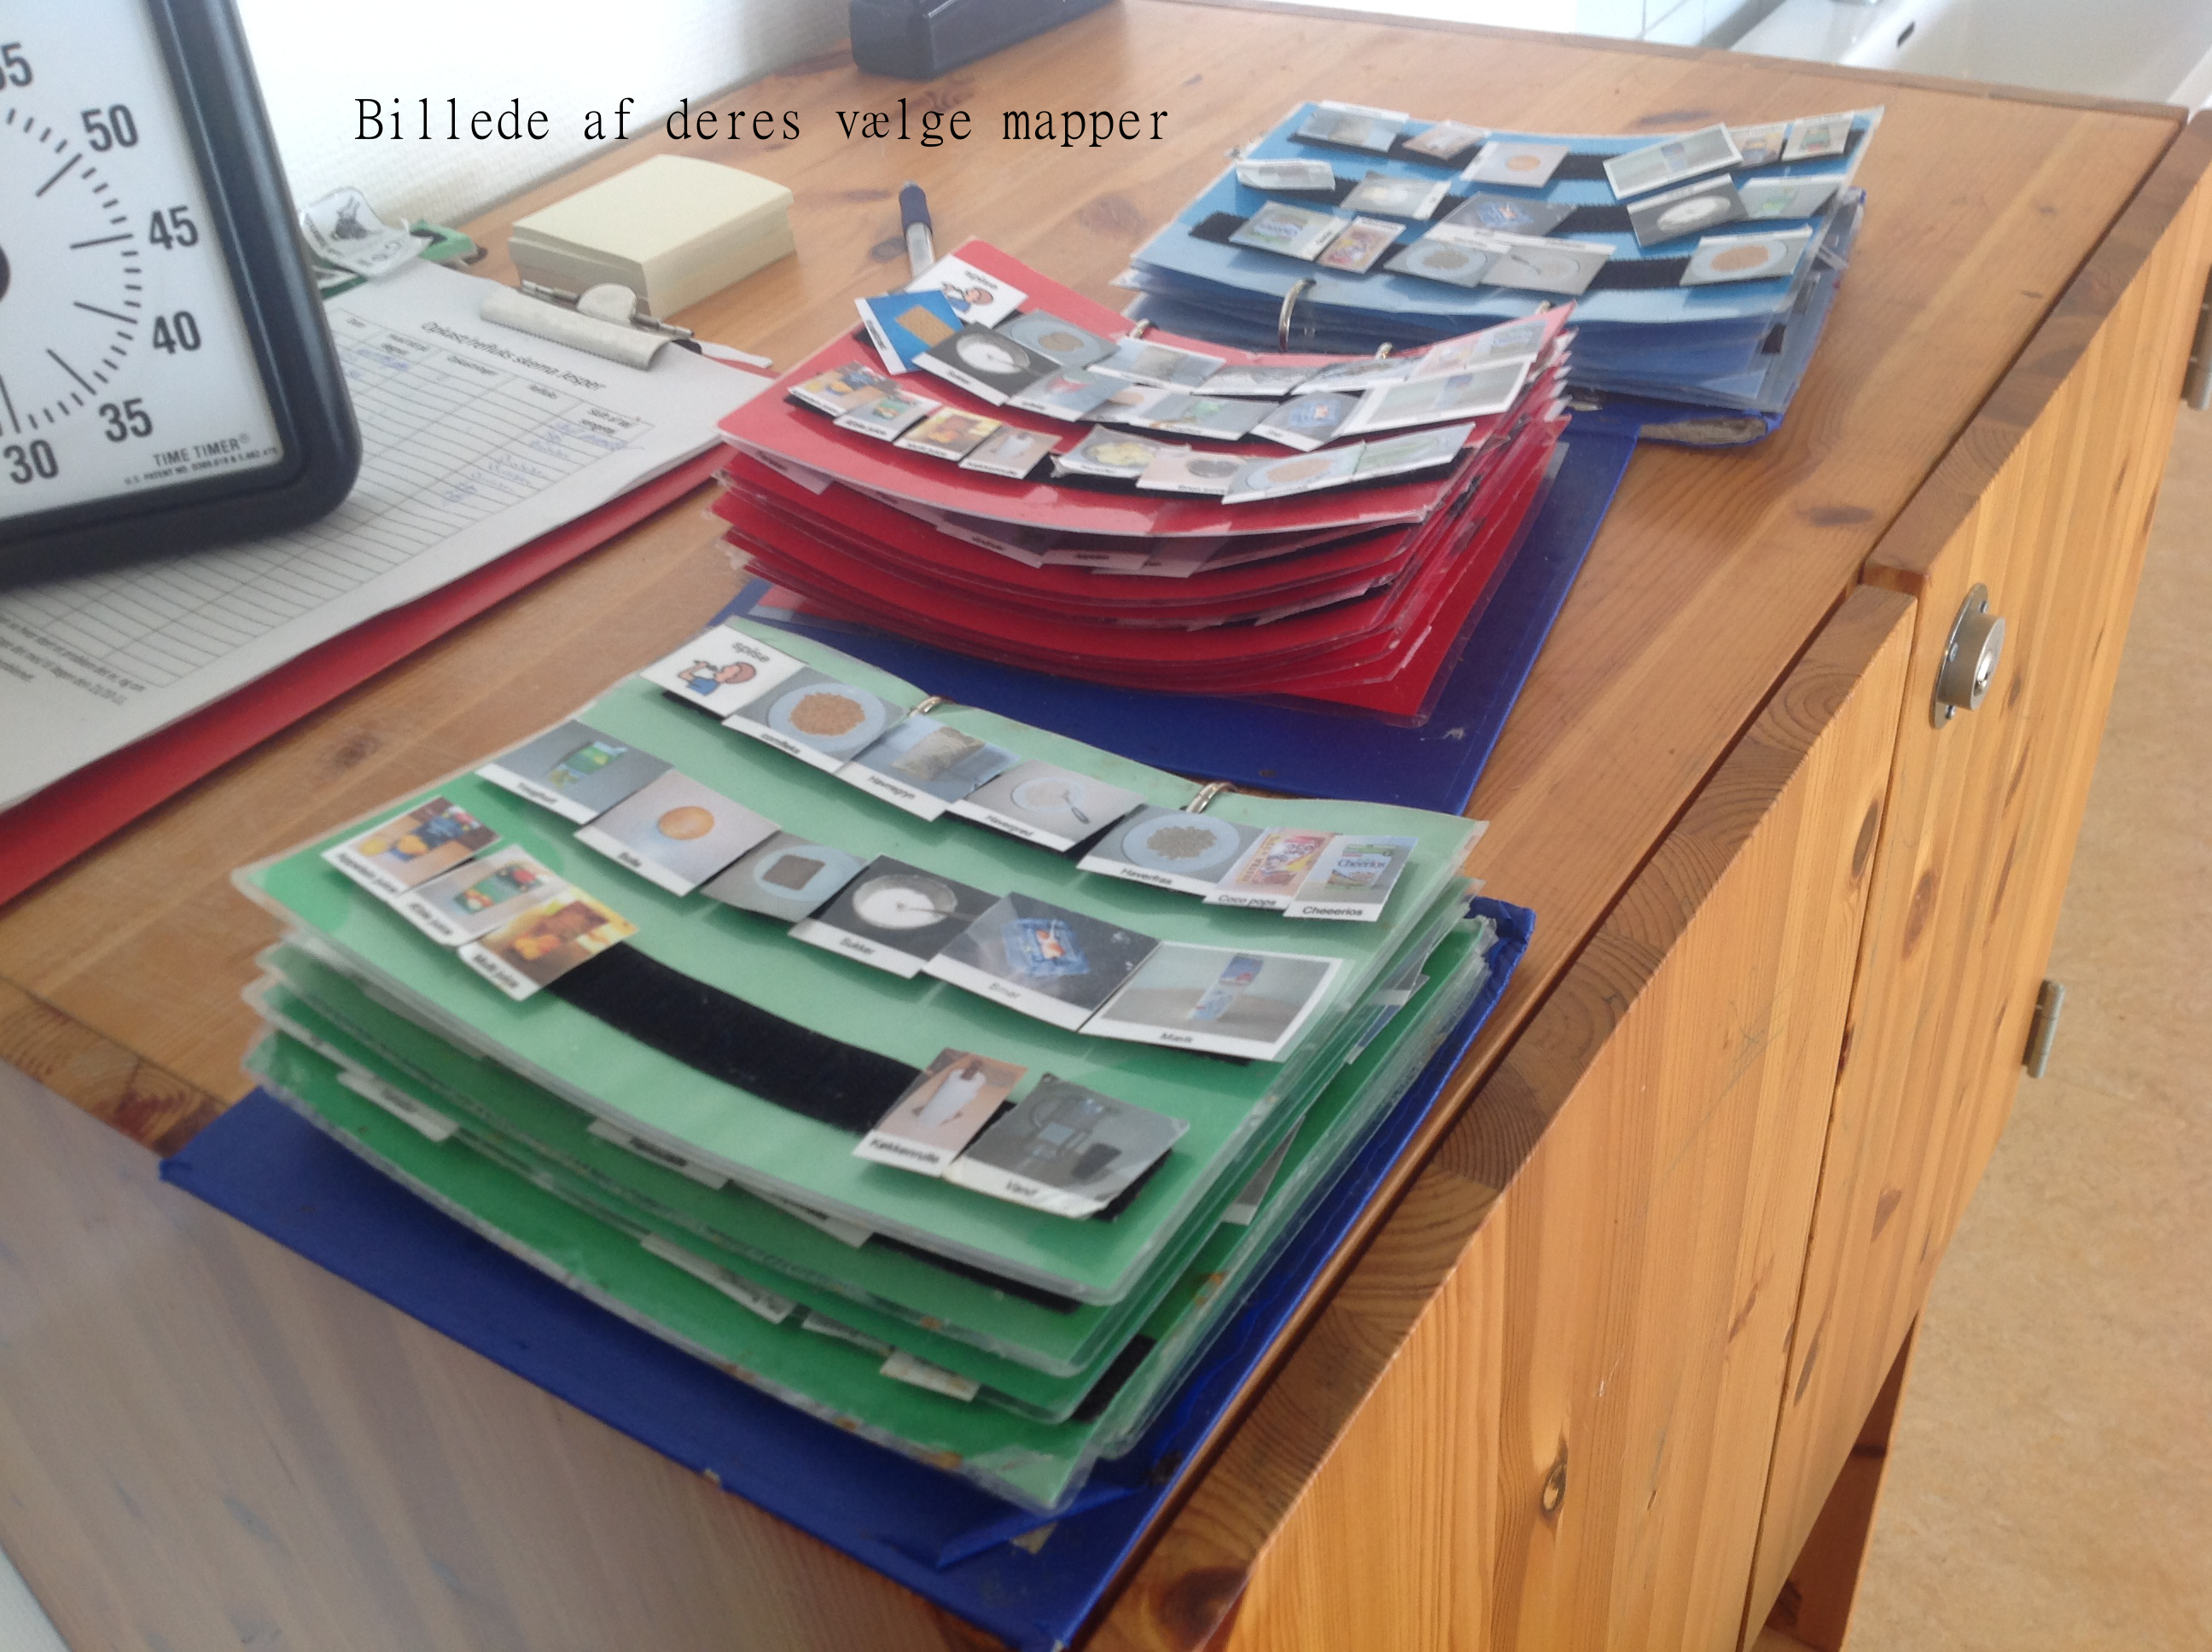
\includegraphics[width=0.6\textwidth]{media/folders}
	\end{figure}
\end{frame}

\begin{frame}
	\frametitle{Motivation}
	\begin{figure}
		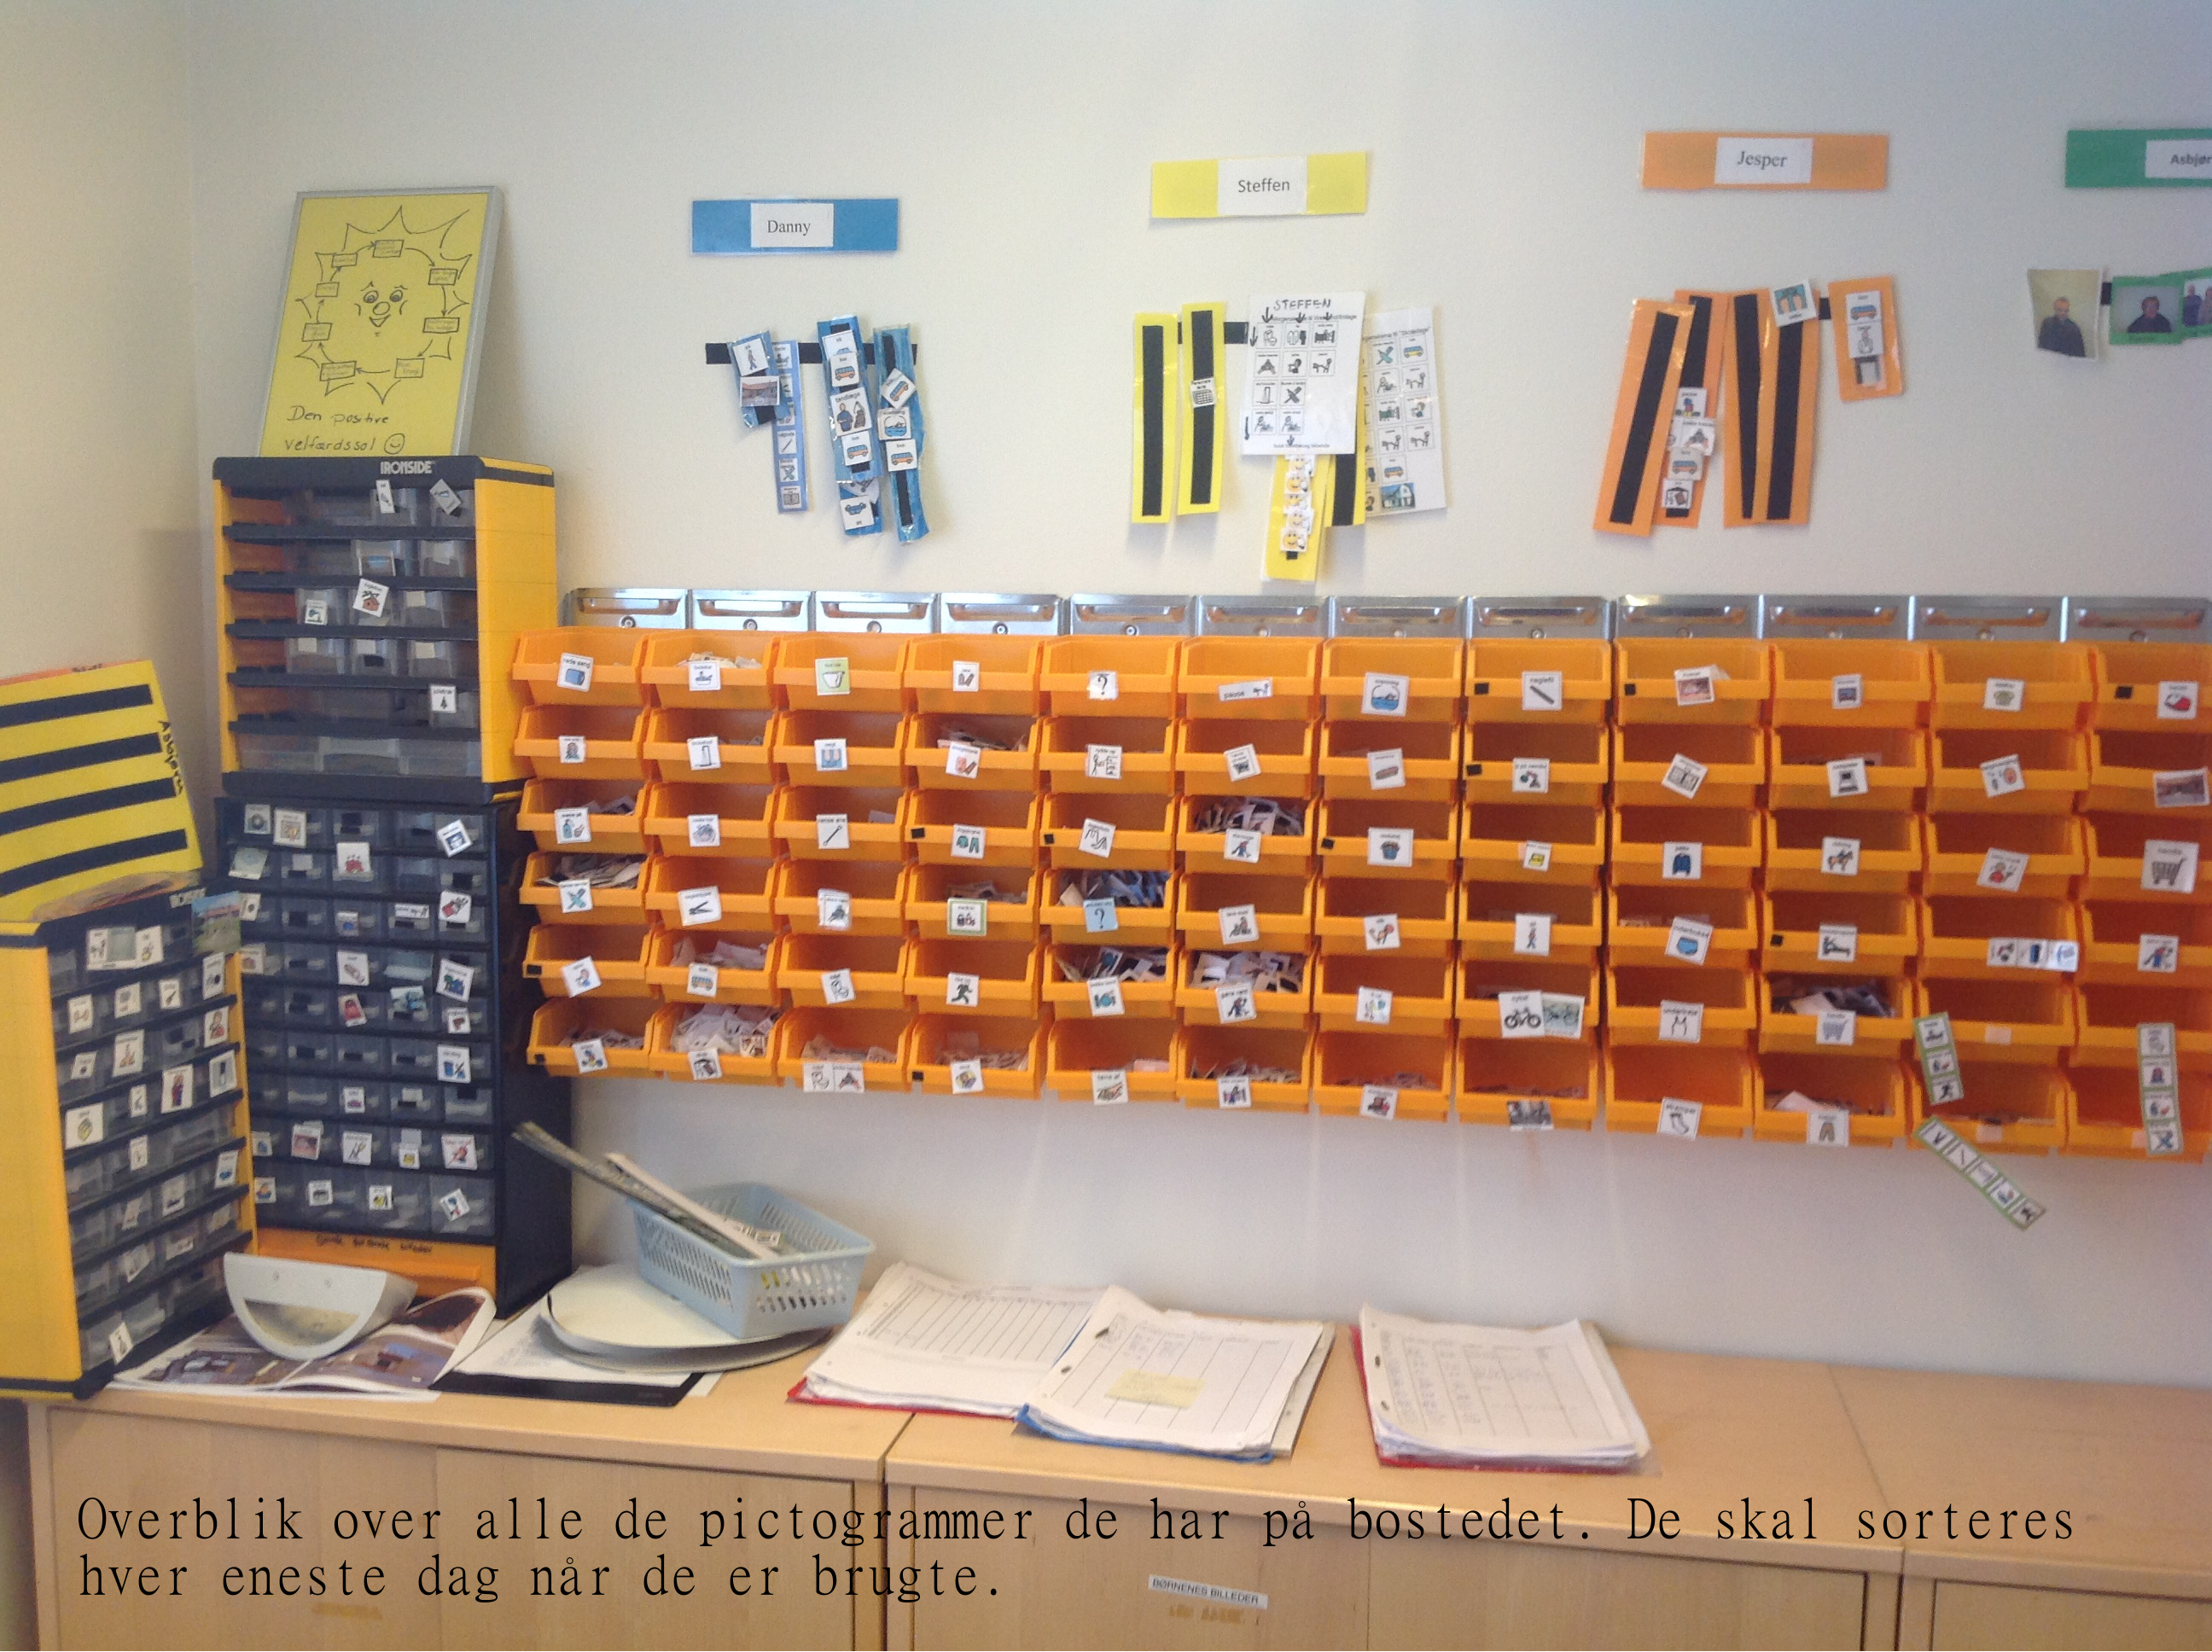
\includegraphics[width=0.5\textwidth]{media/Sortering}		
		\hfill
		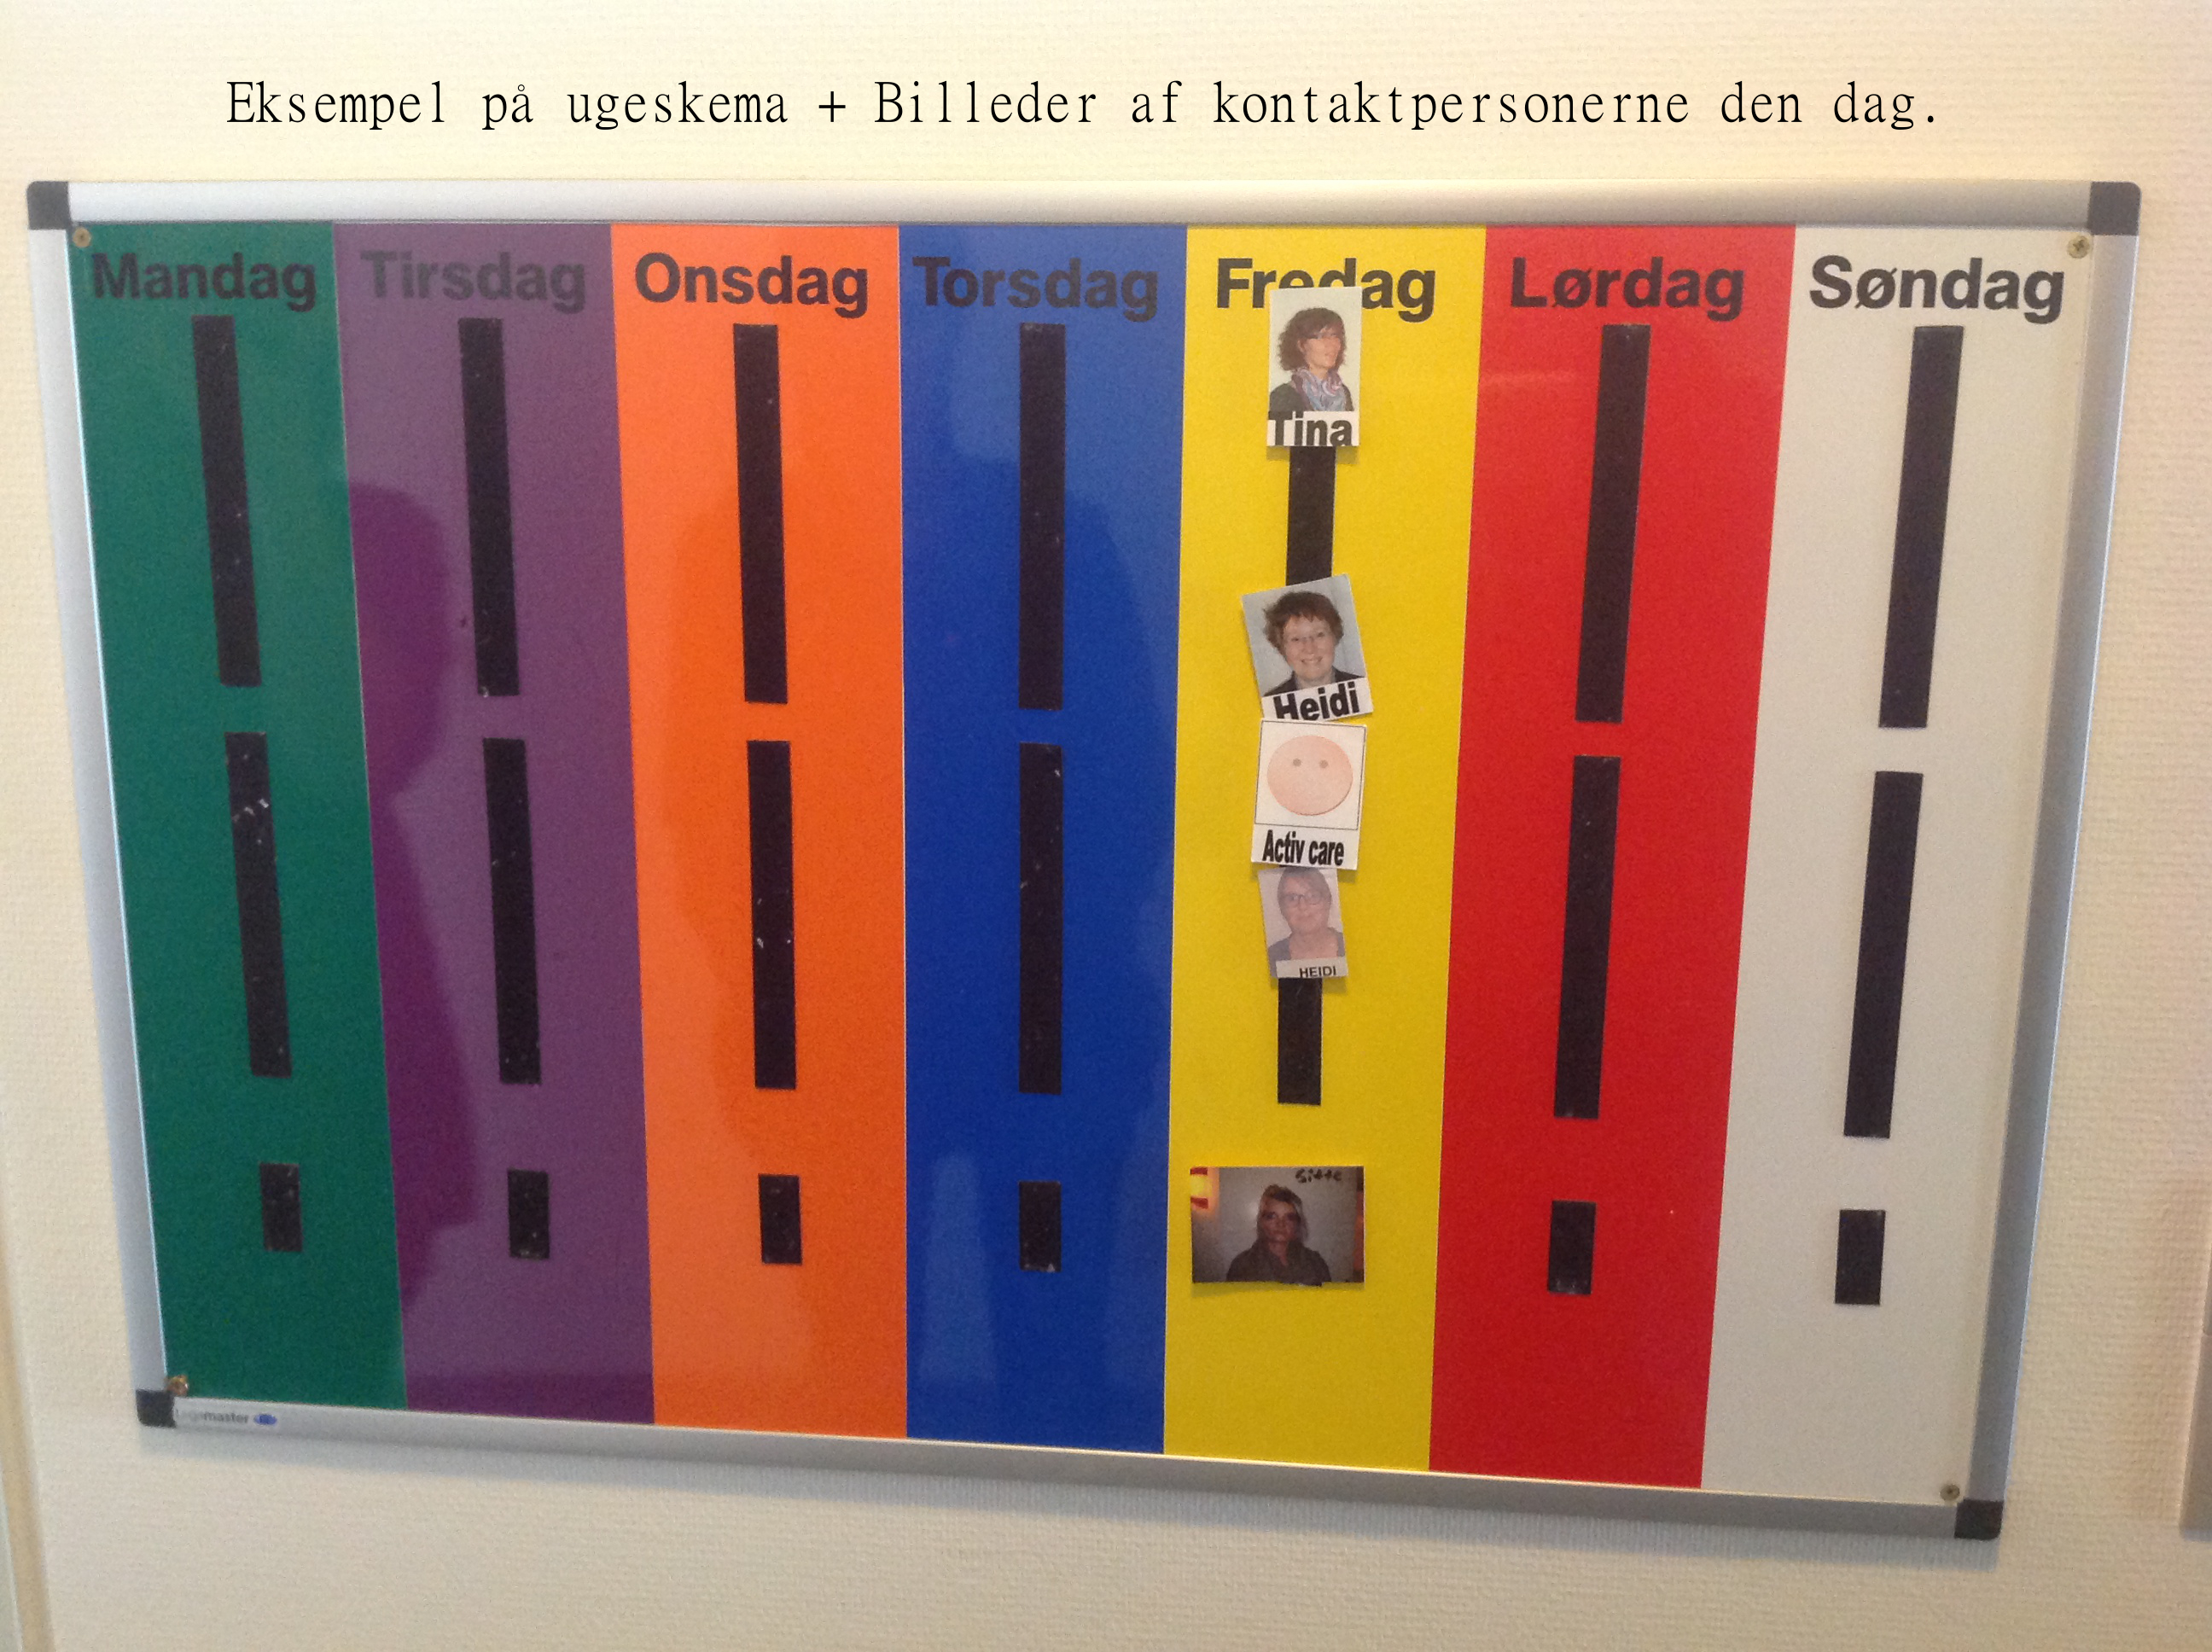
\includegraphics[width=0.5\textwidth]{media/skema}
	\end{figure}
\end{frame}

\begin{frame}
	\frametitle{Multi-Project}
	\begin{itemize}
		\item GIRAF
		\item Previous development projects
		\item Real customers
	\end{itemize}
\end{frame}
	
	
	
\section{Pictogram Creation Tool}
\begin{frame}
	\frametitle{Pictogram Creation Tool}
	\begin{itemize}
		\item Motivation
		\begin{itemize}
			\item Fast pictogram creation
			\item Database usage
		\end{itemize}
		\item Pictogram creation
		\item Existing functionality
	\end{itemize}
	\begin{figure}
		\includegraphics[width=0.5\textwidth]{media/CrocOldCanvas}
		\hfill
		\includegraphics[width=0.42\textwidth]{media/Destroyed}
	\end{figure}
\end{frame}
%new features - als
%-rotate
%-resize
%-collision
%-design changes
%	-record
%	-cam 
%	-save


\section{Key Changes}
\begin{frame}
	\frametitle{Key Changes}
	\begin{itemize}
		\item Rotation of entities
		\item Collision detection
		\item Resizing of entities
		\item Design changes
		\begin{itemize}
			\item Record Dialogue
			\item Camera Dialogue
			\item Save Dialogue
		\end{itemize}
	\end{itemize}
\end{frame}

\begin{frame}
	\frametitle{Rotation}
	\begin{itemize}
	\item Before: Resize Icon not clickable, but worked.
	\item After, use rotation matrix: $R = \begin{bmatrix}
			cos\, \theta & - sin\, \theta\\
			sin\, \theta & cos\, \theta
			\end{bmatrix}$
	\item Rotate point $p = \begin{bmatrix}x\\y\end{bmatrix}$ around (0,0) to get $p'$
	\item $p' = R*p$
	\item Solved Rotation issue with collision detection correctly implemented for rotated entities.
	\end{itemize}
\end{frame}



\begin{frame}
	\frametitle{Collision Detection - Rectangle}
	ABP, BCP, CDP, and DAP all right turns.
		\begin{figure}
		\centering
			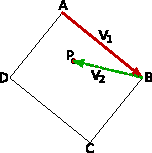
\includegraphics[width=0.6\textwidth]{media/rectangle-collision}
		\end{figure}
\end{frame}

%\begin{frame}
%	\frametitle{Collision Detection - Ellipsis}
%		\begin{figure}
%		\centering
%			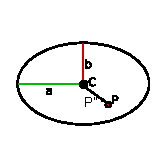
\includegraphics[width=0.6\textwidth]{media/ellipse-collision}
%		\end{figure}
%		$$\frac{ (P''_x * cos(\alpha) - P''_y * sin(\alpha))^2}{a^2} + \frac{(P''_x * sin(\alpha) - P''_y * cos(\alpha))^2}{b^2} \leq 1$$
%\end{frame}

\begin{frame}
	\frametitle{Resize}
	\begin{itemize}
		\item Old version: When resizing just add dragvector components to width and height.
		\item Was bad with "large" rotations
		\item New version:
		\begin{itemize}
			\item More stable
			\item Still "floats" a bit, but acceptable up to $45 ^\circ$
			\item Let us utilize that when resizing!
		\end{itemize}
	\end{itemize}
\end{frame}

\begin{frame}
	\frametitle{Resize - New Version}
			\begin{figure}
			\centering
				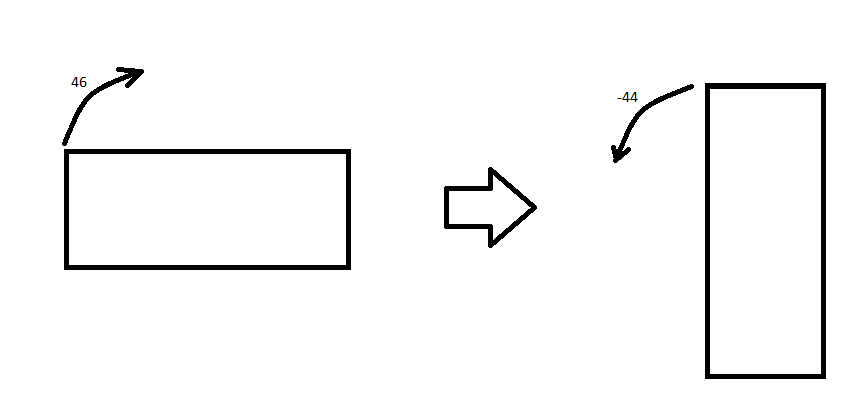
\includegraphics[width=0.6\textwidth]{approach6}
			\end{figure}
			\begin{itemize}
			\item Look at $46^\circ$ as $-44^\circ$
			\item Reset starting point of rectangle
			\item Swap width and height
			\item Then resize with dragvector
			\end{itemize}
			
\end{frame}

\begin{frame}
	\frametitle{Design Changes - Record}
	\begin{figure}
	        \centering
	        \begin{subfigure}[b]{0.24\textwidth}
	                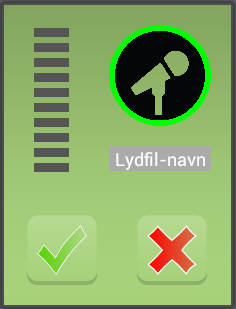
\includegraphics[width=\textwidth]{CrocOldAudio}
	        \end{subfigure}%
	        \begin{subfigure}[b]{0.24\textwidth}
	                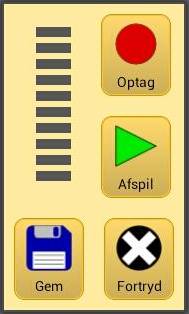
\includegraphics[width=\textwidth]{newrecordidle}
	        \end{subfigure}
	        \begin{subfigure}[b]{0.24\textwidth}
	                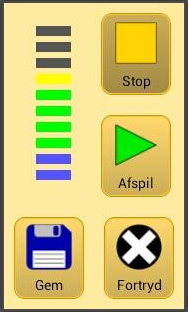
\includegraphics[width=\textwidth]{newrecording}
	        \end{subfigure}
 	        \begin{subfigure}[b]{0.24\textwidth}
 	                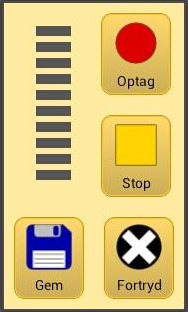
\includegraphics[width=\textwidth]{newrecordplay}
 	        \end{subfigure}
	\end{figure}
\end{frame}

%flere slides til design changes
\begin{frame}
	\frametitle{Design Changes - Camera, old}
	Switch to camera.
		\begin{figure}
		\centering
			\includegraphics[width=0.8\textwidth]{CrocOldCanvas}
		\end{figure}
\end{frame}

\begin{frame}
	\frametitle{Design Changes - Camera, old}
	Take picture.
		\begin{figure}
		\centering
			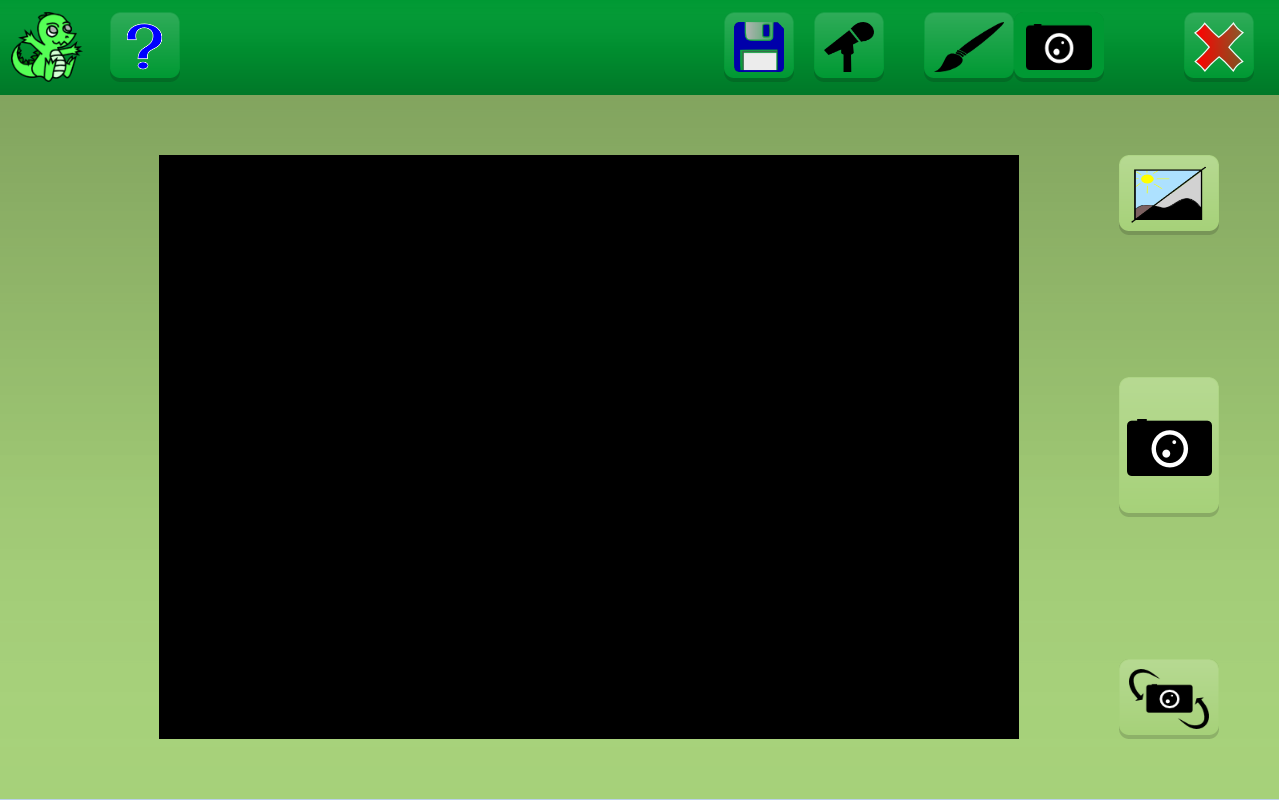
\includegraphics[width=0.8\textwidth]{CrocOldCamera}
		\end{figure}
\end{frame}

\begin{frame}
	\frametitle{Design Changes - Camera, old}
	Load picture.
		\begin{figure}
		\centering
			\includegraphics[width=0.8\textwidth]{CrocOldCanvas}
		\end{figure}
\end{frame}

\begin{frame}
	\frametitle{Design Changes - Camera, old}
	Load picture.
		\begin{figure}
		\centering
			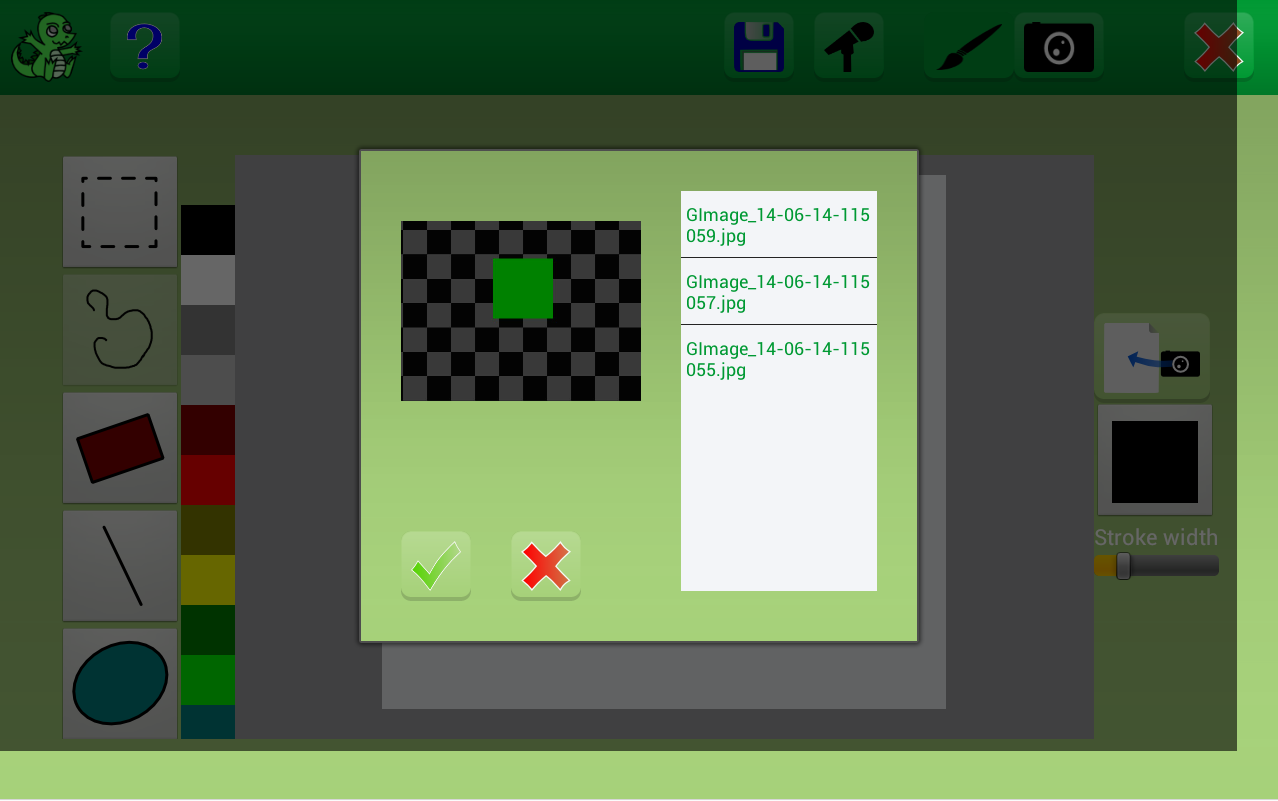
\includegraphics[width=0.8\textwidth]{cameraload}
		\end{figure}
\end{frame}
%flere slides til design changes
\begin{frame}
	\frametitle{Design Changes - Camera}
	\begin{itemize}
		\item Old way was deemed unintuitive
		\item Customers wanted a way to take pictures similar to other camera apps
		\item Inspiration from Instagram and iOS camera app
	\end{itemize}
\end{frame}

\begin{frame}
	\frametitle{Design Changes - Camera, new}
	Open Camera
		\begin{figure}
		\centering
			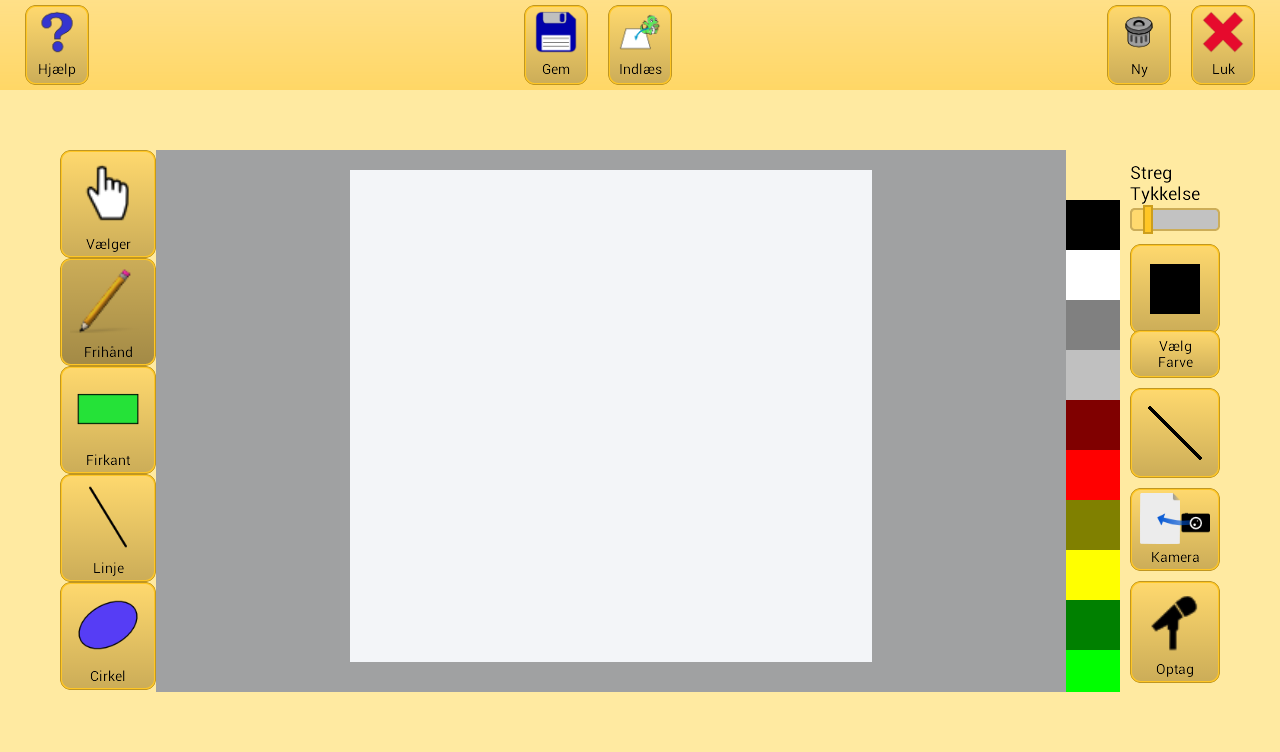
\includegraphics[width=0.8\textwidth]{final-main-ui}
		\end{figure}
\end{frame}

\begin{frame}
	\frametitle{Design Changes - Camera, new}
	Take picture
		\begin{figure}
		\centering
			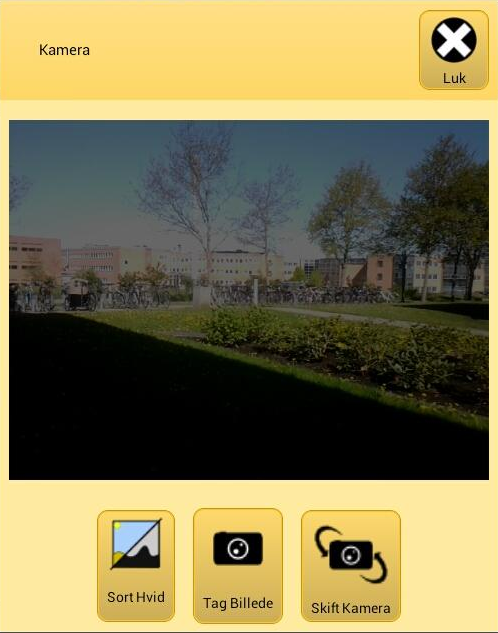
\includegraphics[width=0.5\textwidth]{cam1}
		\end{figure}
\end{frame}

\begin{frame}
	\frametitle{Design Changes - Camera, new}
	Accept picture
		\begin{figure}
		\centering
			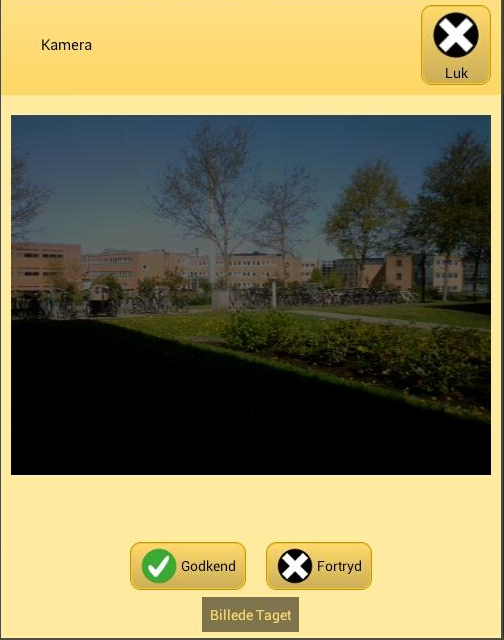
\includegraphics[width=0.5\textwidth]{cam2}
		\end{figure}
\end{frame}

\begin{frame}
	\frametitle{Design Changes - Camera, new}
	Result
		\begin{figure}
		\centering
			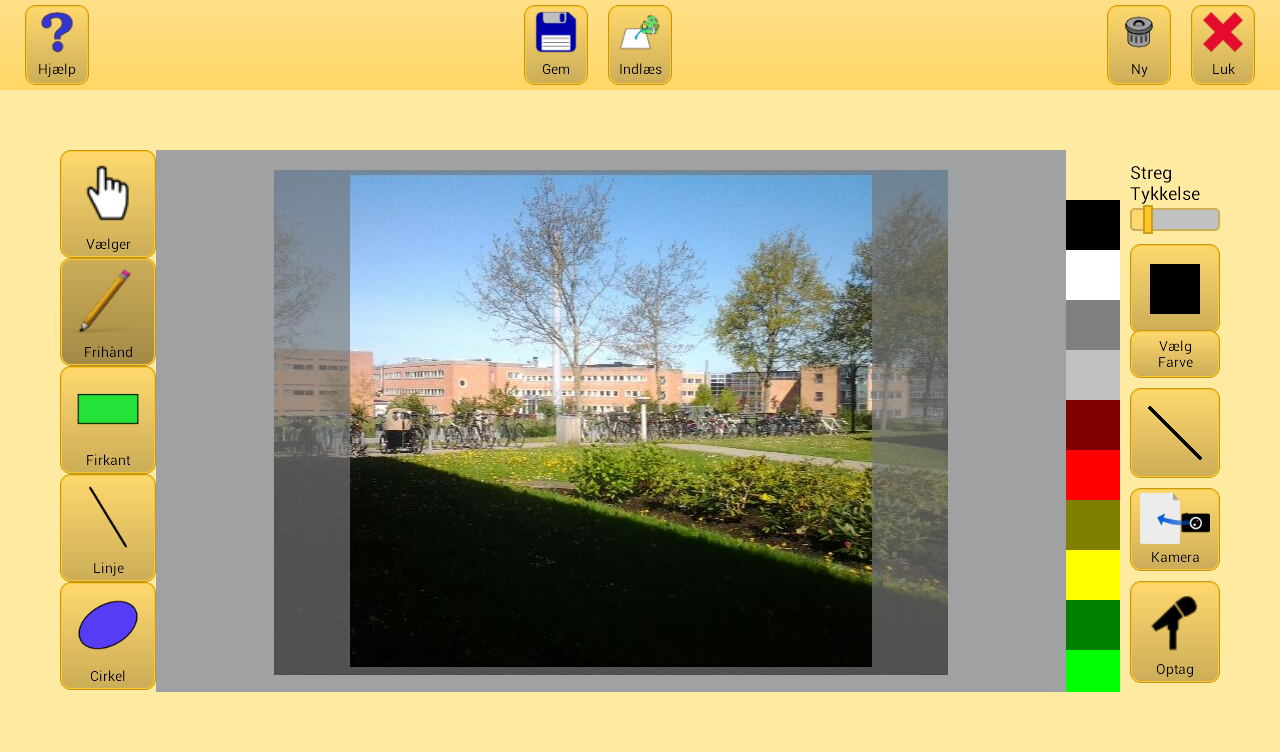
\includegraphics[width=0.8\textwidth]{cam3}
		\end{figure}
\end{frame}
%flere slides til design changes
\begin{frame}
	\frametitle{Design Changes - Save Dialogue}
	\begin{itemize}
	\item Database not finished previous years
	\item A Dialogue was made, but functionality to save was not.
	\item Now able to save pictograms as the database got developed.
	\end{itemize}
\end{frame}

\begin{frame}
	\frametitle{Design Changes - Save, Old}
		\begin{figure}
		\centering
			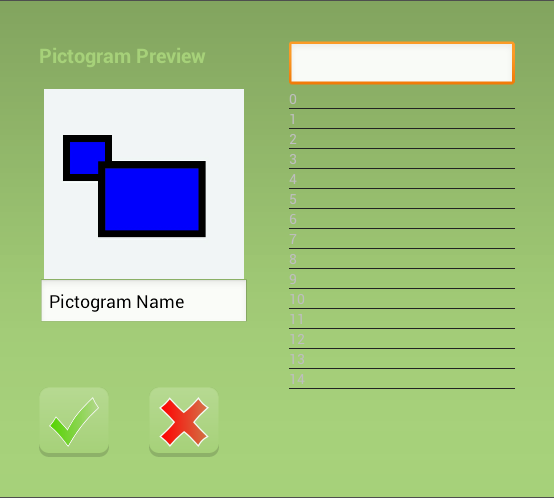
\includegraphics[width=0.8\textwidth]{saveold}
		\end{figure}
\end{frame}

\begin{frame}
	\frametitle{Design Changes - Save, New}
		\begin{figure}
		\centering
			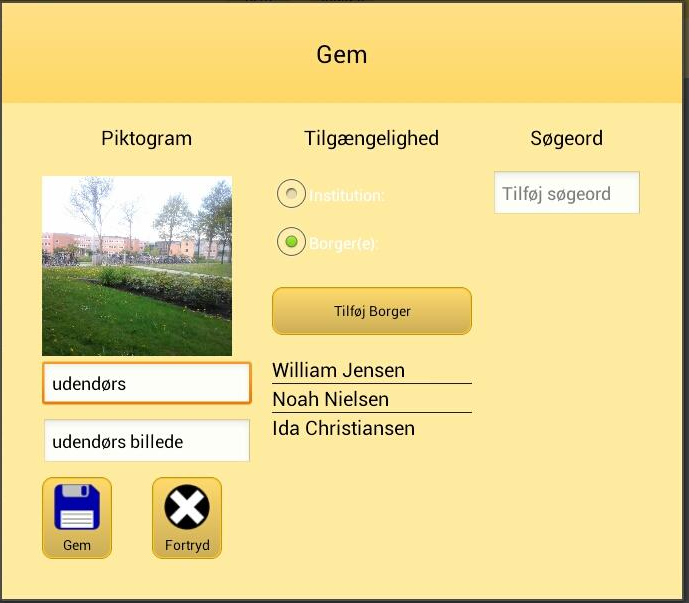
\includegraphics[width=0.8\textwidth]{savenew}
		\end{figure}
\end{frame}
	\section{Demonstration}
	
		\begin{frame}
			\frametitle{Demonstration}
			\begin{center}
				Demonstration
			\end{center}
		\end{frame}	
		
	\section{Usability Test}
		\begin{frame}
			\frametitle{Usability Test}
			\begin{itemize}
				\item Two testees
				\item Tasks
				\item Instant Data Analysis
			\end{itemize}
		\end{frame}
		
		\begin{frame}
			\frametitle{Tasks}
			\begin{itemize}
				\item "Take a black-and-white picture"
				\item "Record audio"
				\item "Save a pictogram"
			\end{itemize}
		\end{frame}
		
		\begin{frame}
			\frametitle{Results}
			\begin{itemize}
				\item Nine categorised usability problems
				\begin{itemize}
					\item Playing sound - Cosmetic
					\item Drawing entities - Serious
					\item Pushing entities back - Critical
				\end{itemize}
			\end{itemize}
		\end{frame}

	

	
	\section{Media Library Collaboration}
		\begin{frame}
		\frametitle{Media Library Collaboration}
		\begin{itemize}
			\item MediaPlayer
			\item Text to Speech
			\item Collaboration experience
		\end{itemize}

		\end{frame}
		
	

	\section{Reflections}
		\begin{frame}
		\frametitle{Reflections}
		\begin{itemize}
			\item Usability test experience gain
			\item SCRUM experience
			\item Customer interaction
			\item Further Development
		\end{itemize}
		More points to be added
		\end{frame}


	\bgroup
	\setbeamercolor{background canvas}{bg=black}
	\begin{frame}[plain]{}
	\addtocounter{framenumber}{-1}	
		\begin{center}
		%\textcolor{white}{END}
		\end{center}
	\end{frame}
	\egroup
\end{document}
